% \documentclass{cumcmthesis}
\documentclass[withoutpreface,bwprint]{cumcmthesis} %去掉封面与编号页,电子版提交的时候使用。


\usepackage[framemethod=TikZ]{mdframed}
\usepackage{url}   % 网页链接
\usepackage{subcaption} % 子标题
\usepackage{algorithm}
\usepackage{algorithmicx}
\usepackage{algpseudocode}
\usepackage{amsmath}
 
\floatname{algorithm}{算法}
\renewcommand{\algorithmicrequire}{\textbf{输入:}}
\renewcommand{\algorithmicensure}{\textbf{输出:}}

\title{一个测量装置在大规模制造中的标定问题}

\begin{document}

\maketitle

\begin{center}
    522031910677\quad 杨锦畅
    
    \kai{日期:2024年4月7日}
\end{center}

{\heiti 摘要:}本文提出了一个解决大规模制造中非线性元件标定问题的方法。采用改良的双种群遗传算法,将传统的单向个体流动转变为双向优质个体交流,结合自适应参数调整解决成本和生产效率优化问题。引入基于Bayes公式干预的变异概率控制方法,通过赋予基因片段不同的变异率来提高优质个体生成概率。同时,应用多种优化策略提升代码效率,为解决相似问题提供了可借鉴的技巧。此外。本文对遗传算法中轮盘赌、锦标赛、截断、随机遍历四种不同的选择算法进行了对比实验和讨论。

{\heiti 关键词:}双种群遗传算法;遗传参数自适应;选择算法比较

%\tableofcontents

%\newpage

\section{模型假设}
\begin{enumerate}
    \item \textbf{虽然不同传感器的性质有一定随机性,但存在一种规律能够描述整体的$V-T$走势。}如果每组数据的走势均为随机(如温度传感器的温敏器件不同),则分析测试点的位置没有意义。
    \item \textbf{题目给出的成本可以作为真实成本的评价依据。}其他可能的成本可以被忽略。
    \item \textbf{题目所给数据均为精确数据,可以作为模型判断依据和训练根据。}
\end{enumerate}
\section{符号说明}

\begin{center}
    \begin{tabular}{cccccc}
        \toprule
        \makebox[0.3\textwidth][c]{符号}  &  \makebox[0.5\textwidth][c]{意义} \\ \midrule
        $N$ & 种群规模\\
        $X,Y$ & 种群总体X和Y\\
        $f(x_i)$ & 第i个个体的适应度\\
        $P$ & 概率参数向量\\
        $s_{i,j}$ & 第i个个体,第j个待测温度点的误差成本\\
        $T_{i,j}$ & 第i个个体,第j个待测温度点的精确温度\\
        $\hat{T_{i,j}}$ & 第i个个体,第j个待测温度点的预测温度\\
        \bottomrule
    \end{tabular}
\end{center}
注:以上为本论文中涉及的重要通用符号,对于少量具体问题中的具体符号会在使用时进行解释。

\section{问题分析}
本题是一个典型的组合优化问题,需要从90个可行的温度点中找出有限个点进行标定,使得成本最优化。由于目标单一,且解的总集有限,故考虑采用遗传算法进行问题求解。
\newpage
针对该解决方案,需要建立的数学模型有:
\begin{itemize}
    \item \textbf{测定点集模型},在此例中将其看作一个由90位二进制数组成的基因序列,用0/1表示该温度是否进行标定。
    \item \textbf{成本评价模型},在此例中由题目给出,对每个测定点集可以计算平均成本,视作其适应度。
\end{itemize}

进行成本计算前,需要得到完整的温度-电压方程,而标定所直接得到的数据是若干个离散的点。因此,需要进行插值操作。根据对数据的初步分析,考虑采用三次样条插值方法补全未测定的温度点电压数据。

\section{模型建立与求解}
%使用logical数组、persistent数据进行优化,由于polyfit对数据数量级的要求,将电压单位转化为V进行拟合,关于参数选取
%关于变异:先解释为什么常规的变异是不可行的,然后推出基于贝叶斯公式干预的变异控制
%使用矩阵运算插值实现效率优化(可以测试效率,包括其他优化手段,但不是重点)
%不同的选择规则
%不同的变异概率控制,对比收敛效率
%另一种自适应变异概率(文件传输助手截图)
\subsection{简单遗传算法}

\subsubsection{基本思想}
遗传算法(Genetic Algorithm, GA)是一种经典的仿生算法,通过矩阵模拟种群,而个体对应的向量则对应着一组解。在此题中,使用长度为90的logical向量表示一个解,其中值为true则表示该温度点被选择,反之表示其不被选择。在简单遗传算法中,对于每一代种群,需要经过评估、选择、交叉、变异四个操作,产生新一代种群。
\begin{enumerate}
    \item \textbf{评估}。要使种群趋向更优,首先需要了解每个个体的“适应度”。此步骤对种群的所有个体进行适应度评估,通过适应度函数计算出当前种群的适应度向量,并记录当前最大适应度和最优个体。
    \item \textbf{选择}。以轮盘赌算法为例(其余选择算法将在拓展研究中讨论),每个个体$x_i$被选入新种群的概率$p(x_i)$等于其适应度$f(x_i)$在种群所有个体适应度之和中的占比,即
    \begin{equation}\label{eqn-1}
    p(x_i)=\frac{f(x_i)}{\sum_{j=1}^N f(x_j)}
    \end{equation}
    式中,N表示种群规模。共进行N次选择,即可生成一个新的种群,其适应度期望应当优于原种群。
    \item \textbf{交叉}。经过选择,种群中会存在很多相同的个体,此时为了个体的多样性,需要进行交叉和变异操作。本例中采取两点交叉的算法,随机生成两个介于1至90之间的整数l和r,对两个个体$x_i$和$x_j$的l至r基因片段进行交换,如图\ref{fig:exchange}。
    \begin{figure}[htbp]
        \centering
        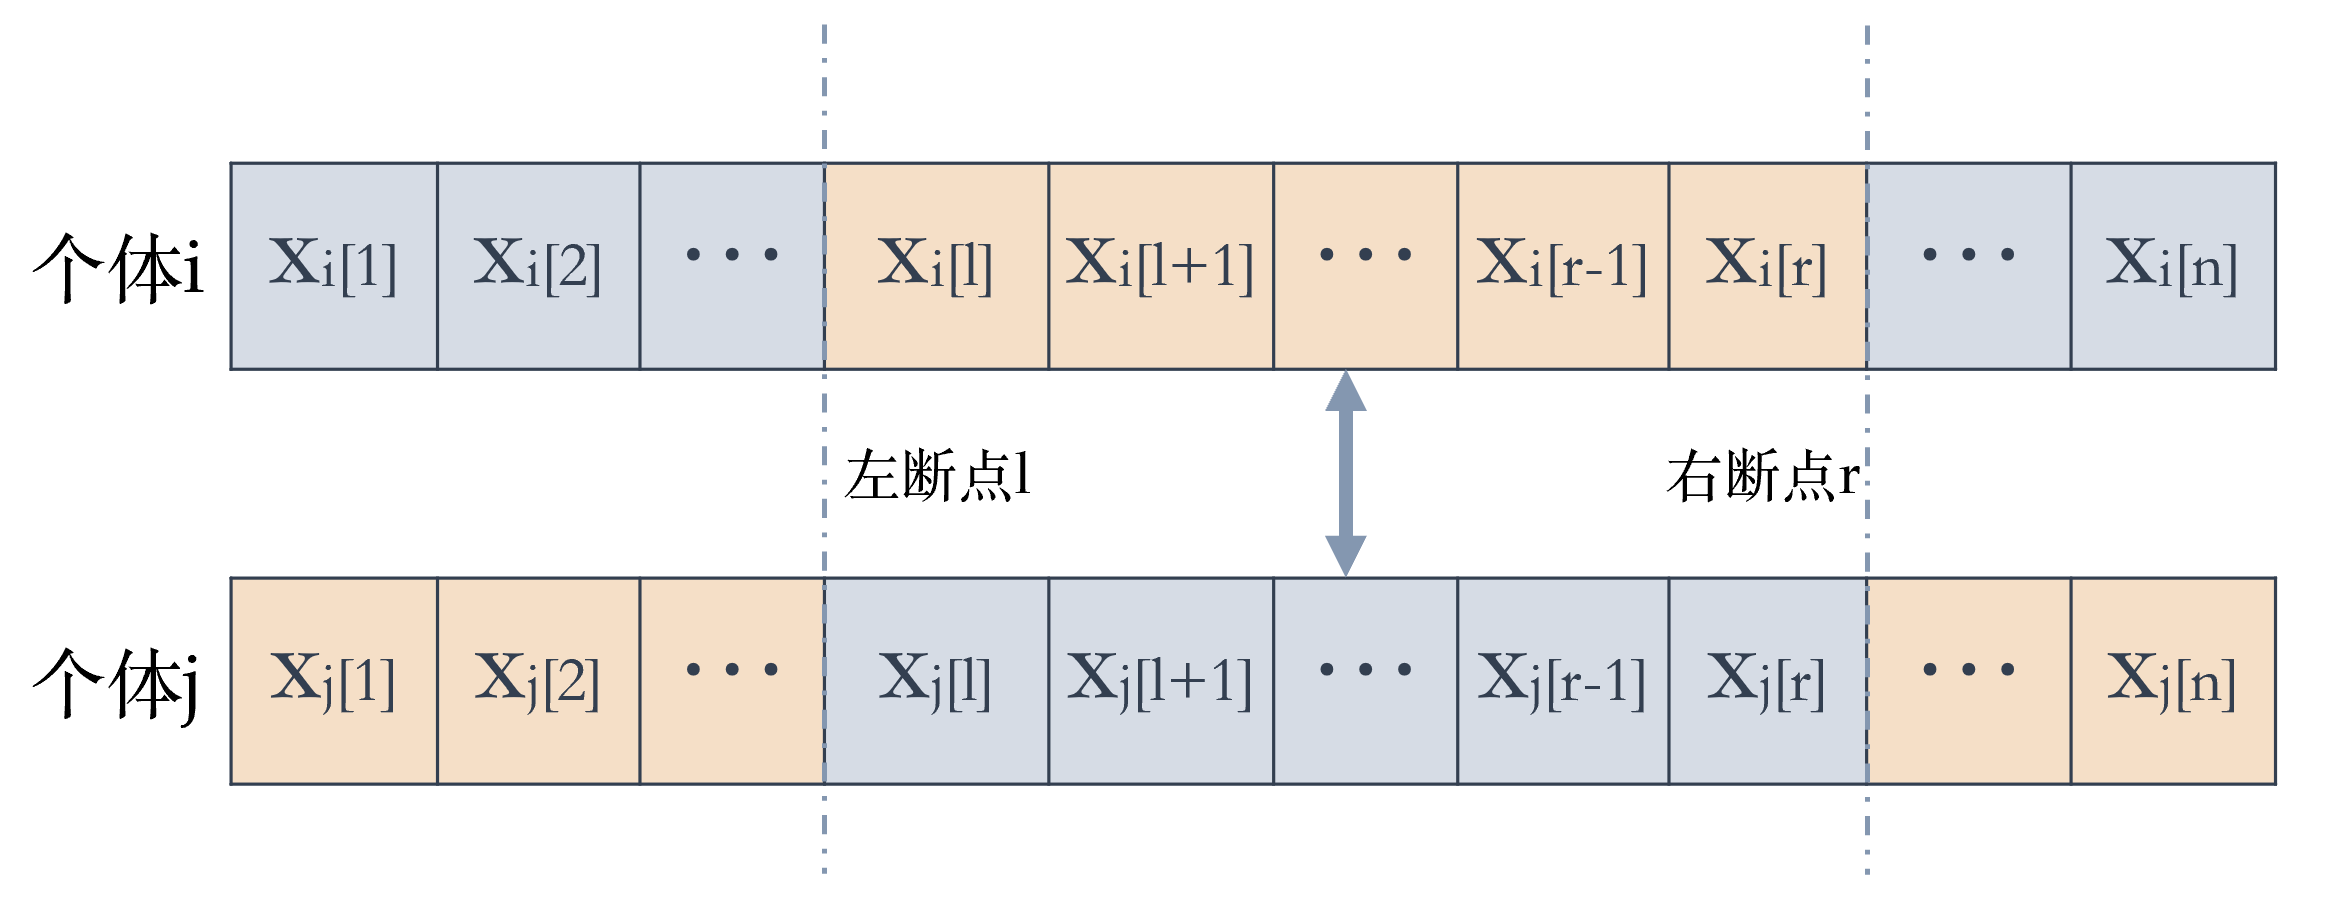
\includegraphics[width=0.75\linewidth]{CUMCMThesis-master//figures/两点交叉.png}
        \caption{两点交叉算法示意}
        \label{fig:exchange}
    \end{figure}
    本例中,采取对相邻个体进行交叉的策略,即$j=i+1$。
    \item \textbf{变异}。在较为成熟的种群中,会有大量相同的个体,此时交叉不能提供任何多样性。设置一定的变异概率$p_v$,对任意个体的任意基因,都有一定概率取反。在基础的算法中,$p_v$是一个定值,但对变异概率的调整优化在本例中对算法收敛速度和“早熟”情况的避免都起着至关重要的作用,后文中将对其进行讨论。
\end{enumerate}

设置迭代次数或终止条件(如k代以内没有出现更优个体),即可通过遗传算法计算出大部分优化类问题的较优解。

\subsubsection{适应度计算}

本例中的适应度在要求中给出,计算方法可分为以下几步:

\begin{enumerate}
    \item 根据个体i选定的标定温度及其对应的电压,对训练集中所有条目,通过三次样条插值\cite{spline},预测所有待测电压对应的温度,记为$\hat{T_{i,1}},\hat{T_{i,2}},\cdots,\hat{T_{i,n}}$。
    \item 计算总成本$C_{total}$,其值由\ref{eqn-2}式给出。
    \begin{equation}\label{eqn-2}
        C_{total}=QkN+\sum_{i=1}^N \sum_{j=1}^{90} s_{i,j}
    \end{equation}
    式中,Q=80,表示一次标定的成本;k表示个体中true的数量,即每次完整标定的次数;$s_{i,j}$由\ref{eqn-3}式给出。
    \begin{equation}\label{eqn-3}
    s_{i,j}=
    \left\{\begin{matrix}
    0\\
    1\\
    10\\
    30\\
    80000
    \end{matrix}\right.
    \begin{matrix}
    \left | \hat{T_{i,j}}-T_{i,j} \right | \le 0.5\\
    0.5<\left | \hat{T_{i,j}}-T_{i,j} \right | \le 1.0\\
    1.0<\left | \hat{T_{i,j}}-T_{i,j} \right | \le 1.5\\
    1.5<\left | \hat{T_{i,j}}-T_{i,j} \right | \le 2.0\\
    \left | \hat{T_{i,j}}-T_{i,j} \right | >2.0
    \end{matrix}
    \end{equation}
    \item 计算适应度$f(x_i)$,为了进一步拉开优质个体与其他个体之间的差距、加速收敛,采取对平均成本统一减去400后再取倒数的策略,即
    \begin{equation}\label{eqn-4}
        f(x_i)=\frac{1}{\frac{C_{total}}{N}-400}
    \end{equation}
\end{enumerate}

\subsection{改进的双种群遗传算法}

双种群遗传算法(Dual Population Genetic Algorithm, DPGA)\cite{dualpop}是对简单遗传算法的一种优化。该算法设置了两个相对独立而又互相交流的种群,能更好地保持多样性、一定程度上避免早熟,也能通过最优个体的交流加快收敛。算法的流程如图\ref{fig:dualpopillus},对两个种群分别初始化、评估、选择、交叉、变异,在此基础上增加“移民”操作。

移民,即间隔一定代数(本例中取5代),用一个种群的最优个体替代另一个种群的最劣个体。常规的双种群遗传算法一般采用“淘汰种群”的概念,仅将该种群的最优个体转移到常规种群中;而针对此优化问题,采取改进的双种群遗传算法,设置两个平等的种群,互相用最优个体替代对方的最劣个体,更好地促进种群之间的交流,加速优化进程。
\begin{figure}[htbp]
    \centering
    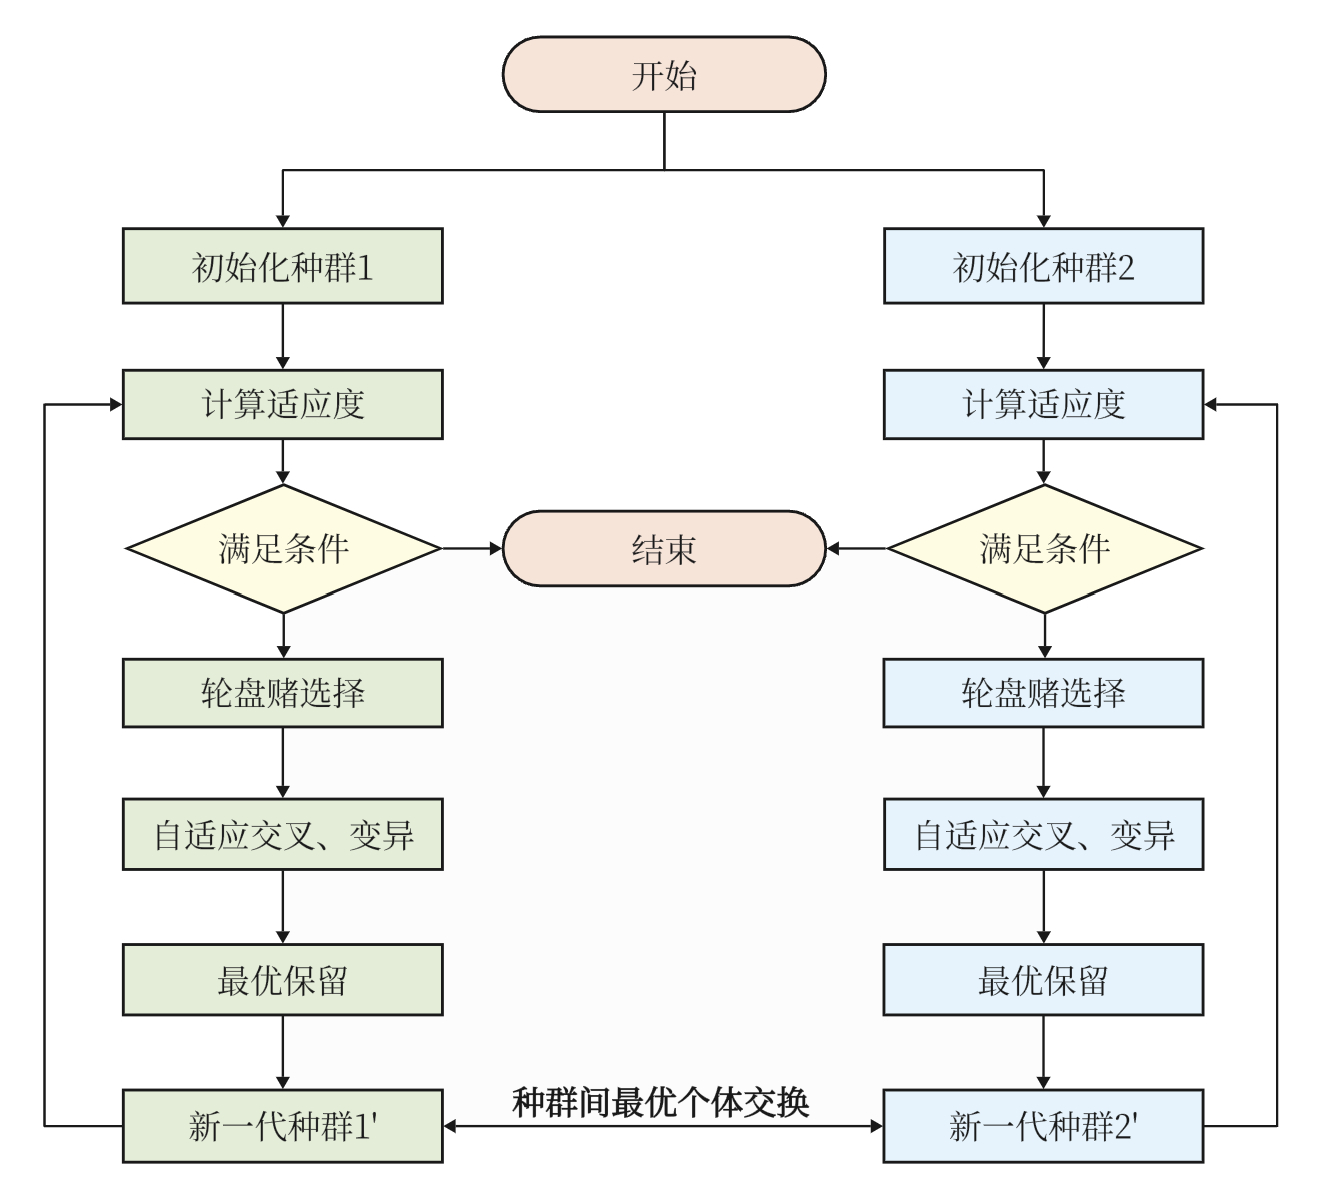
\includegraphics[width=0.53\linewidth]{CUMCMThesis-master//figures/双种群示意.png}
    \caption{双种群遗传算法示意}
    \label{fig:dualpopillus}
\end{figure}

改进的双种群遗传算法伪代码见算法\ref{alg:dualpop}。

\begin{algorithm}[htbp]
    \caption{改进的双种群遗传算法}
    \begin{algorithmic}[1] %每行显示行号
        \Require 适应度函数F,选择函数S,代数G,种群大小N,概率参数向量P
        \State $X,Y \gets randomized\ matrix$
        \For{$g = 1 \to G$}
            \State $fitval1,fitval2 \gets F(X),F(Y)$
            \State $newX,newY\gets S(fitval1,X),S(fitval2,Y)$
            \For{$i = 1 \to N\ Step\ 2$}
                \If {$rand()<P(crossover)$}
                    \State $l,r \gets randi(1,90)$
                    \State $newX(i,l:r) \leftrightarrow newX(i+1,l:r)$
                    \State $newY(i,l:r) \leftrightarrow newY(i+1,l:r)$
                \EndIf
            \EndFor
            \For{$(i,j) = (1,1) \to (N,90)$}
                \If {$rand()<P(mutation)$}
                    \State $newX(i,j)\gets \neg newX(i,j)$
                    \State $newY(i,j)\gets \neg newY(i,j)$
                \EndIf
            \EndFor
            \State $newX(1),newY(1)\gets best\ individual\ of\ X,Y$
            \If{$g\equiv 0(mod\ 5)$}
                \State $newX\gets best\ individual\ of\ Y$
                \State $newY\gets best\ individual\ of\ X$
            \EndIf
        \EndFor
    \end{algorithmic}
    \label{alg:dualpop}
\end{algorithm}

\newpage

\subsection{参数的确定和优化}

\subsubsection{种群规模}
\label{sec:popsize}

本例中,单个个体由90位0/1表示,为了确保多样性,避免陷入局部最优,应当设置较大的种群规模N(N代表单个种群的个体数量,即实际算法中总个体数为2N)。考虑到过大的N会导致计算量增加、运行效率降低,故设计实验确定一个较佳的种群规模,测试50代以内某规模所得到解与最优解的接近程度、时间成本和稳定性。测试平台为AMD Ryzen 6800U(电池模式),Matlab R2023b。实验重复五次,表\ref{tab:Nexp}中的数据系五次实验的统计值。

\begin{table}[htbp]
    \centering
    \caption{种群规模确定实验数据}
    \begin{tabular}{cccc}
    \toprule
        种群规模N & 平均完成时间(s) & 最佳成本 & 成本总体标准差$\sigma$ \\
    \midrule
        100 & 211 & 468.86 & 7.4\\
        150 & 309 & 466.37 & 5.6\\
        200 & 407 & 458.97 & 2.8\\
        250 & 503 & 458.97 & 2.2\\
    \bottomrule
    \end{tabular}
    \label{tab:Nexp}
\end{table}

结合实验结果,综合考虑多种因素,最终确定选用200作为单个种群的规模。此时,设置代数为150时,进行的15轮测试中有12次收敛到458.97。

\subsubsection{自适应交叉率和变异率}

为了进一步避免早熟情况,可以使交叉率和变异率根据当前个体在种群中的情况自适应变化\cite{selfadapt}。为了让处于劣势的个体尽早淘汰、变异,同时减少对优势个体的基因破坏,可以如下设置交叉或变异率。

\begin{equation}\label{eqn-5}
    P=\left\{ 
    \begin{matrix}
        P_1-\frac{(P_1-P_2)(f(x_i)-\bar f)}{f_{max}-\bar f},\  f(x_i)\ge \bar f\\
        P_1,\  f(x_i)< \bar f
    \end{matrix}
    \right.
\end{equation}
式中,$f(x_i)$为待交叉个体的较小适应度值或待变异个体的适应度值,$\bar f$为种群平均适应度,$f_{max}$为种群最大适应度。在本例中,由于问题的搜索空间多达$2^{90}$种,故交叉概率可以设置得较大,从而在一定时间内搜索更多解,因此对于交叉操作,$P_1=1,P_2=0.8$;而变异概率则不能过大(\ref{sec:bayes}中将进一步讨论),设置$P_1=0.05,P_2=0.02$。

\subsubsection{基于Bayes公式干预的变异概率控制}
\label{sec:bayes}

对于变异概率,一般对不同的基因片段内容使用相同的规则。但在本题中,个体中更多的true会导致更高的成本(更低的适应度),且实际上最优解中false的数量是远远多余true的。如果对true和false使用相同的变异概率,假设某个经过选择的种群中true的数量为$G_T$,false的数量为$G_F$,变异概率为p,则变异后种群中true数量的期望$E(G_T')$由\ref{eqn-6}式给出。

\begin{equation}\label{eqn-6}
    E(G_T')=G_F\cdot p+G_T\cdot (1-p)=p(G_F-G_T)+G_T
\end{equation}
这个期望对变异前的$G_T$作商可得\ref{eqn-7}式。
\begin{equation}\label{eqn-7}
    \frac{E(G_T')}{G_T}=p(\frac{G_F}{G_T}-1)+1
\end{equation}

显然,$G_F>G_T$,且$G_F/G_T\gg 1$,因此变异会导致种群中true的数量增多。在此基础上,如果没有选择操作,则种群最终必然趋向true和false数量的平衡。虽然算法中的选择操作会淘汰掉其中的劣势个体,但为了能让淘汰效率对抗变异导致的比例失调,就需要调低变异概率,造成迭代后期多样性不足。

为了解决这个问题,本例采取一种基于Bayes公式干预的变异概率控制。该算法的目标就是使变异过程产生更多趋近最优解的个体,保证种群中true和false数量的合理性。对当前得到的最优个体$X(i)$,记$G_F(i)=g_f,\ G_T(i)=g_t$,如下设置种群中true和false分别变异的概率系数$\rho _t$和$\rho _f$。

\begin{equation}\label{eqn-8}
    \rho_t=\frac{g_f}{g_f+g_t},\quad
    \rho_f=\frac{g_t}{g_f+g_t}
\end{equation}

$\rho_t$和$\rho_f$是关于代数gen的函数。综合\ref{eqn-5}式和\ref{eqn-8}式,可以得到第gen代第i个个体、第j个基因片段的变异概率由\ref{eqn-9}式给出。
\begin{equation}\label{eqn-9}
    p_v(gen,i,j)=\rho \cdot \frac{P(g_t+g_f)}{2g_t}
\end{equation}

\subsection{几种运算效率优化方案}
%开局就用点乘15,使用logical数组,persistent数组,预开数组
为了在算法确定的情况下提高代码的运行速度,本文给出了如下四种针对性优化方案:
\begin{enumerate}
    \item 初始化种群时,使false的数量大于true,提供尽可能更好的初始种群。具体实现上,可以对随机数进行乘方运算后再取整。
    \item 使用logical形式的数组存储种群。由于本例中基因仅由0和1构成,故使用logical数据类型能够在尽可能少占用资源的情况下正常实现功能。
    \item 使用persistent变量存储训练数据。如果每次调用适应度函数都读取一次训练集,会消耗较多时间;global变量则违背模块化编程的思想。使用persistent变量可以避免以上问题。
    \item 在进行任何大型矩阵的赋值前,先将矩阵设置为目标大小的零矩阵。在MATLAB中,修改数据比逐个添加数据效率要高得多。
\end{enumerate}

\subsection{结果展示}

经过多轮运行,得到的最优解为
$$[5\quad 22\quad 45\quad 73\quad 88]$$
其对应的测试集平均成本为458.9685。

对于此最优解和过程中得到的两个次优解进行误差成本稳定性分析,得到图\ref{fig:errplot}。其中,次优解1为$[4\ 22\ 45\ 73\ 88]$,其平均成本为463.52;次优解2为$[4\ 23\ 46\ 74\ 87]$,其平均成本为466.37。分析图像可知,所得的最优解不仅平均成本最低,且误差成本最稳定、高误差出现频率最小、峰值最低。

\begin{figure}[htbp]
    \centering
    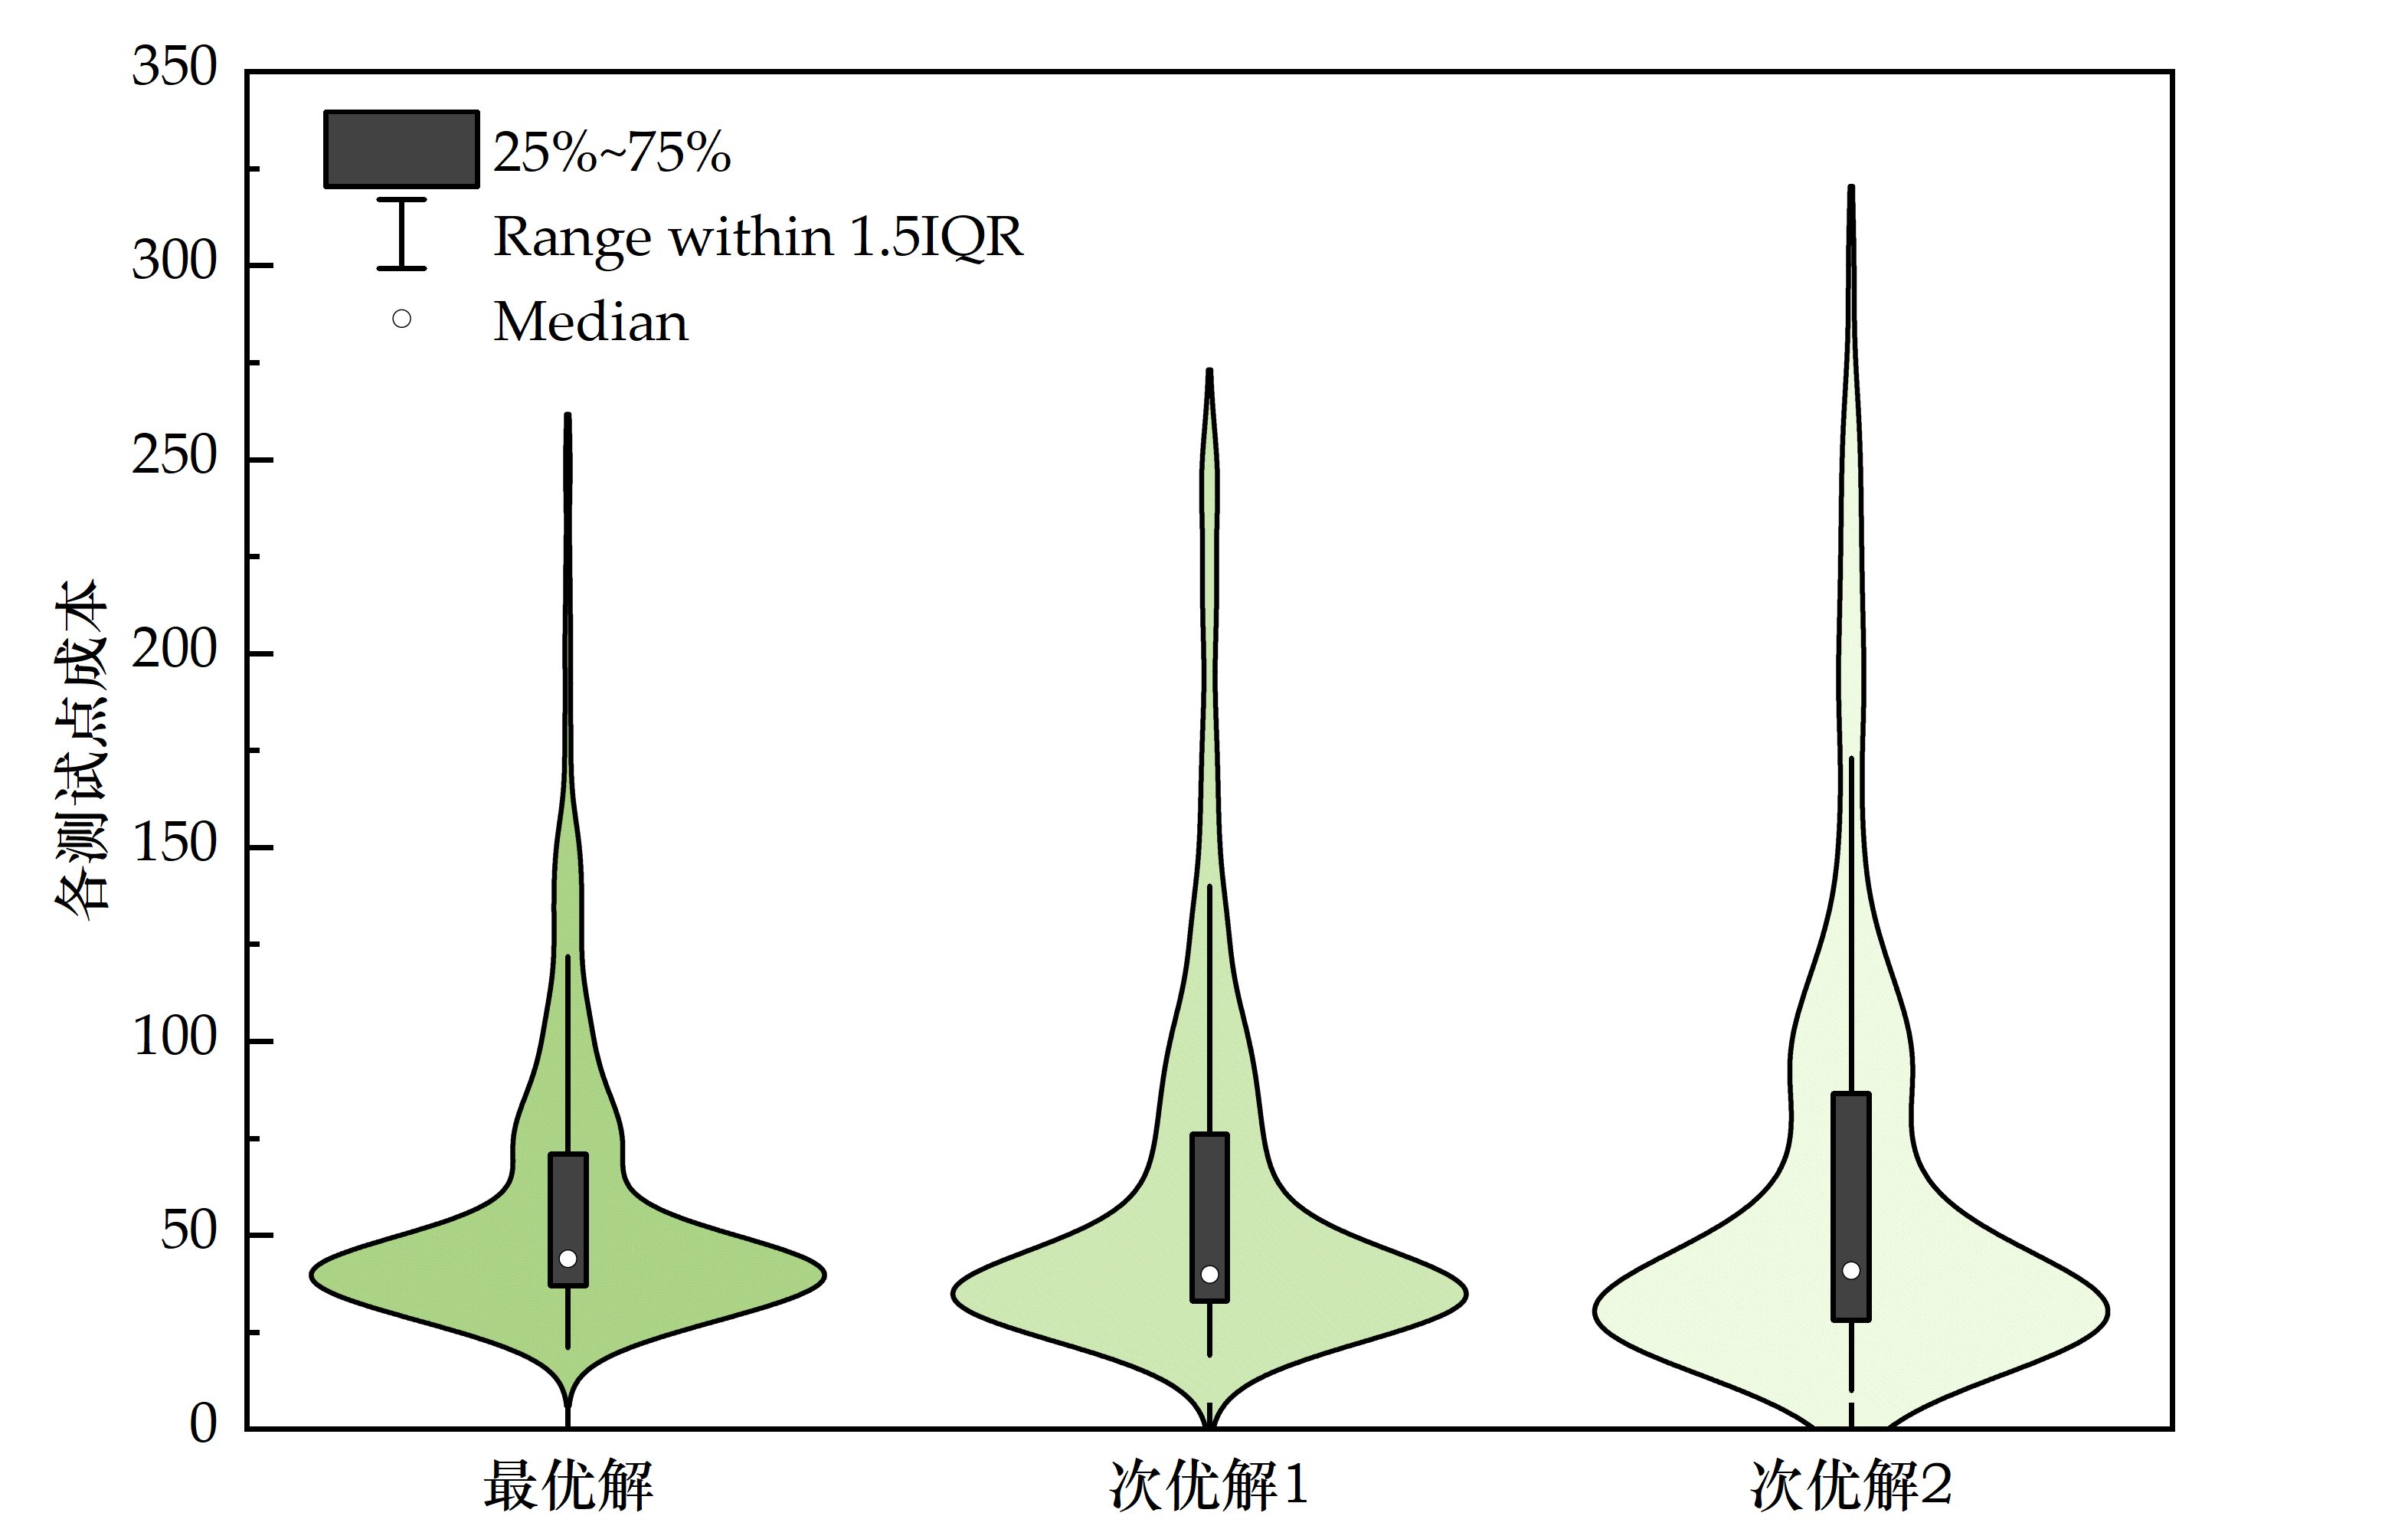
\includegraphics[width=0.65\linewidth]{CUMCMThesis-master//figures/最优解和次优解.png}
    \caption{三个较优解在测试集中的误差成本及其稳定性}
    \label{fig:errplot}
\end{figure}

其中一次收敛至最优解的收敛过程如图\ref{fig:minavg}。在这次收敛过程中,从代数79开始,最优解从6个测试点变为5个测试点,而这也是平均成本由逐渐变小转变为逐渐增大的分界线。其原因可能和\ref{sec:test}中最优解在测试集中表现不佳的原因类似,即5个测试点的个体很容易在某些温度上存在较大误差,而随着5个测试点的精英个体出现,配合\ref{sec:bayes}中提出的变异概率计算方法,种群中5个测试点的个体会逐渐变多,而出现的较大误差点也会增加,导致平均成本不降反增。

\begin{figure}[htbp]
    \centering
    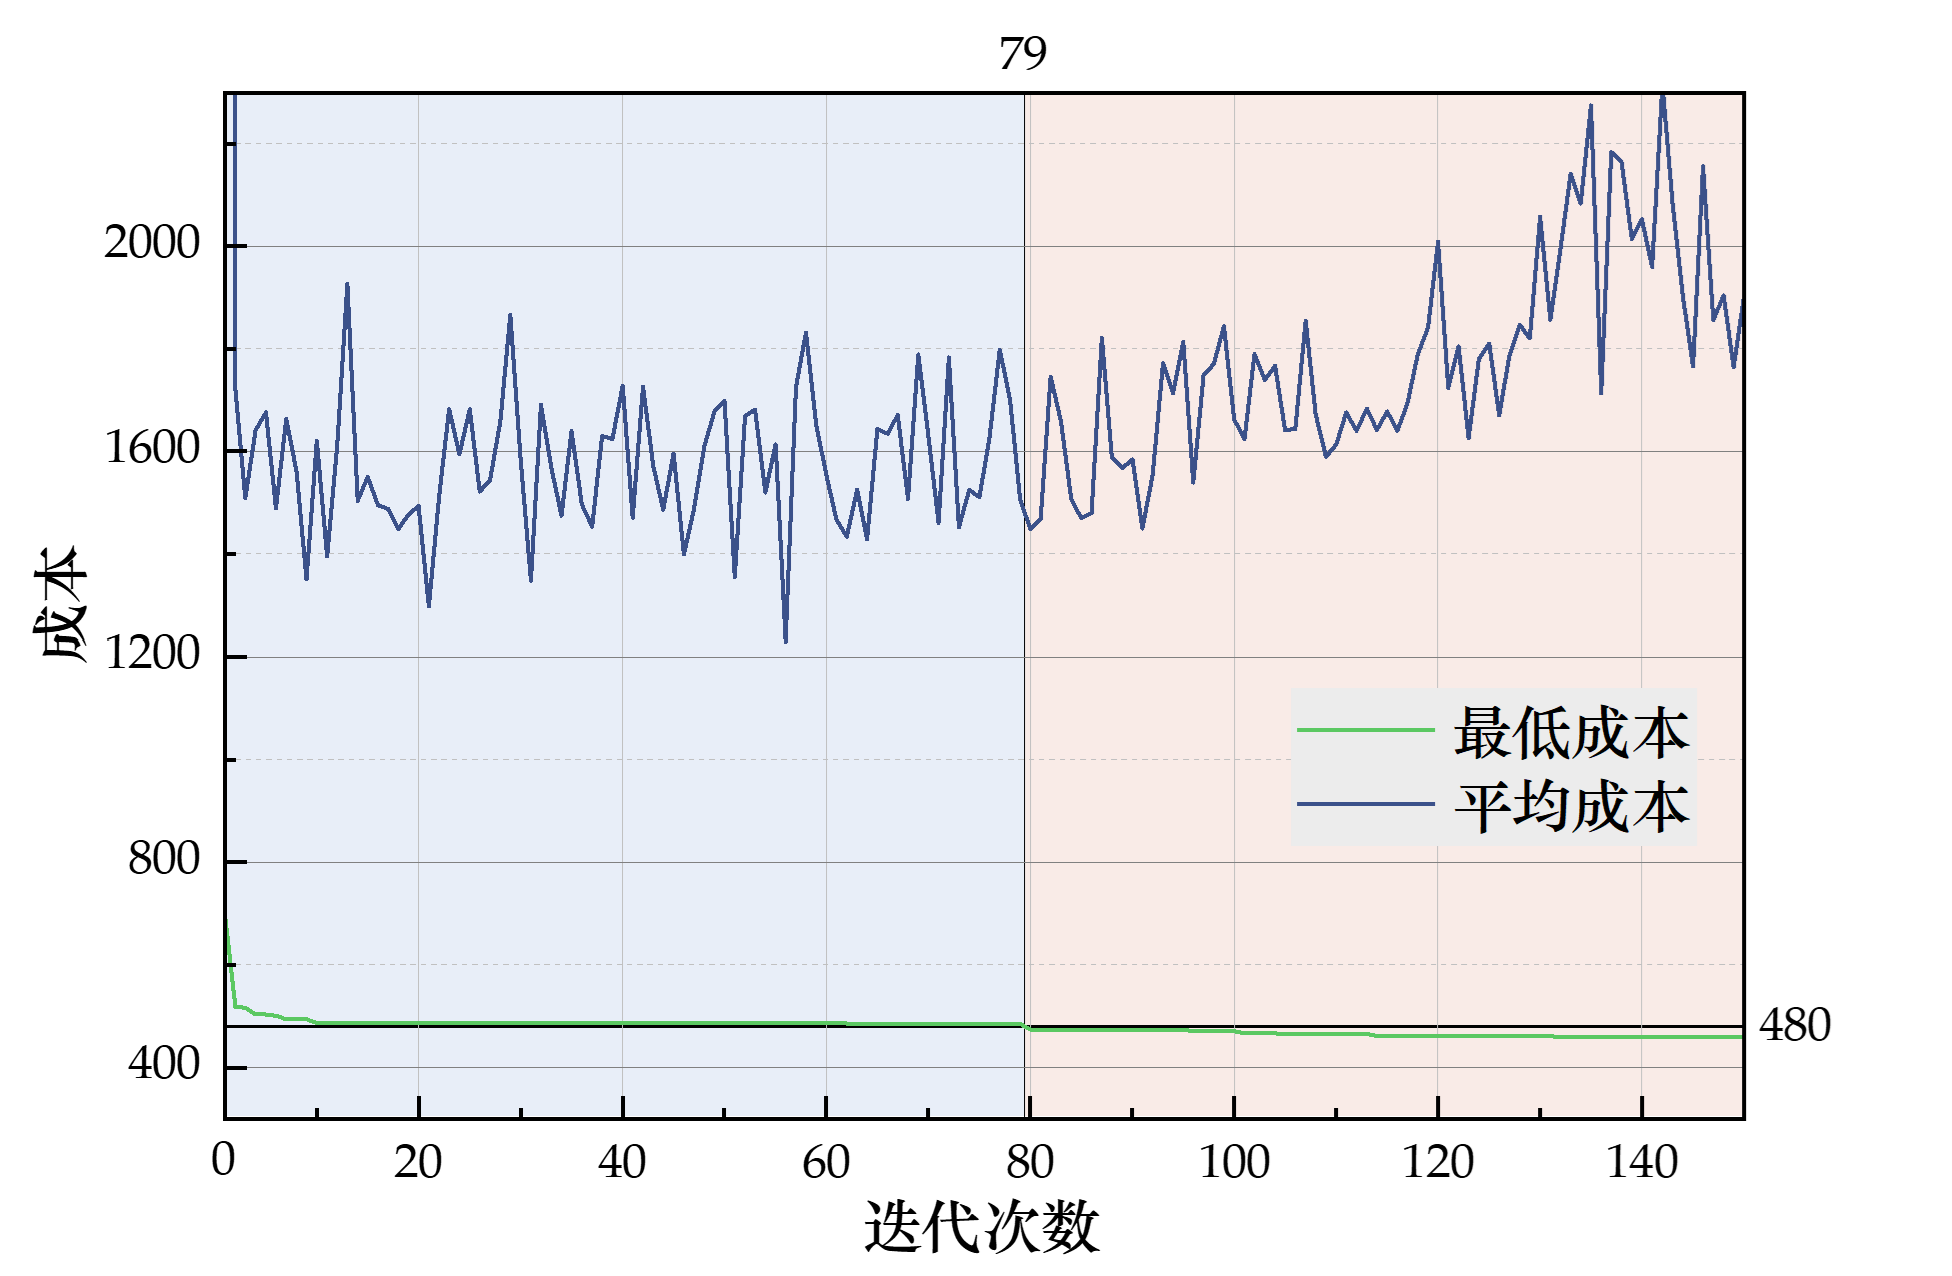
\includegraphics[width=0.75\linewidth]{CUMCMThesis-master//figures/最小和平均.png}
    \caption{一次收敛至最优解的过程}
    \label{fig:minavg}
\end{figure}

\section{模型测试与评价}

\subsection{在测试集中的表现}
\label{sec:test}

使用测试集A和B对上述结果进行测试,所得的平均成本分别为619.62和619.45。这个结果远高于训练集得到的458.97。对每个测试点的成本进行分析,发现在两个测试集中各有一个测试点出现了超过2$^{\circ} \mathrm C$的误差,导致了很大的惩罚值。对其他次优解进行测试,所得平均成本情况如表\ref{tab:test}。

\begin{table}[htbp]
    \centering
    \caption{种群规模确定实验数据}
    \begin{tabular}{cccc}
    \toprule
        次优解 & 训练集平均成本 & 测试集A平均成本 & 测试集B平均成本 \\
    \midrule
        $[4\ 22\ 45\ 73\ 88]$ & 463.52 & 464.64 & 464.36\\
        $[4\ 23\ 46\ 74\ 87]$ & 466.37 & 468.86 & 466.46\\
        $[3\ 12\ 26\ 54\ 73\ 88]$ & 488.67 & 488.54 & 489.36\\
        $[2\ 15\ 24\ 52\ 75\ 87]$ & 485.12 & 485.21 & 485.05\\
    \bottomrule
    \end{tabular}
    \label{tab:test}
\end{table}

从表中可以看出,几个次优解在测试集中的表现都相对稳定。因此,最优解可能存在广义的“过拟合”问题,如果要减小误差,可以增加测试集规模,也可以考虑放弃一定的成本,选用六个测试点的方案进行标定。

\subsection{与简单遗传算法的比较}

为了测试改进的双种群遗传算法相较于简单遗传算法是否确实进步,设置简单遗传算法的种群规模$N'=2N$,以抹平双种群带来的个体数量差距,再进行收敛效率、结果稳定性两方面的测试。测试平台为Intel Core i7-12700H,Matlab R2023b。

\begin{enumerate}
    \item \textbf{收敛效率}。对两种算法分别进行5次测试,每次进行150代,迭代过程中的当前最低成本曲线如图\ref{fig:algocmp}。其中,每代对应的数据为10次测试的均值。虽然简单遗传算法在初期更快得到了一批485左右的较优解,但改进的双种群遗传算法更快得到了五个标定点的解,且得到最优解的次数也明显更多。
    \begin{figure}[htbp]
        \centering
        \begin{minipage}[t]{0.49\linewidth}
            \centering
            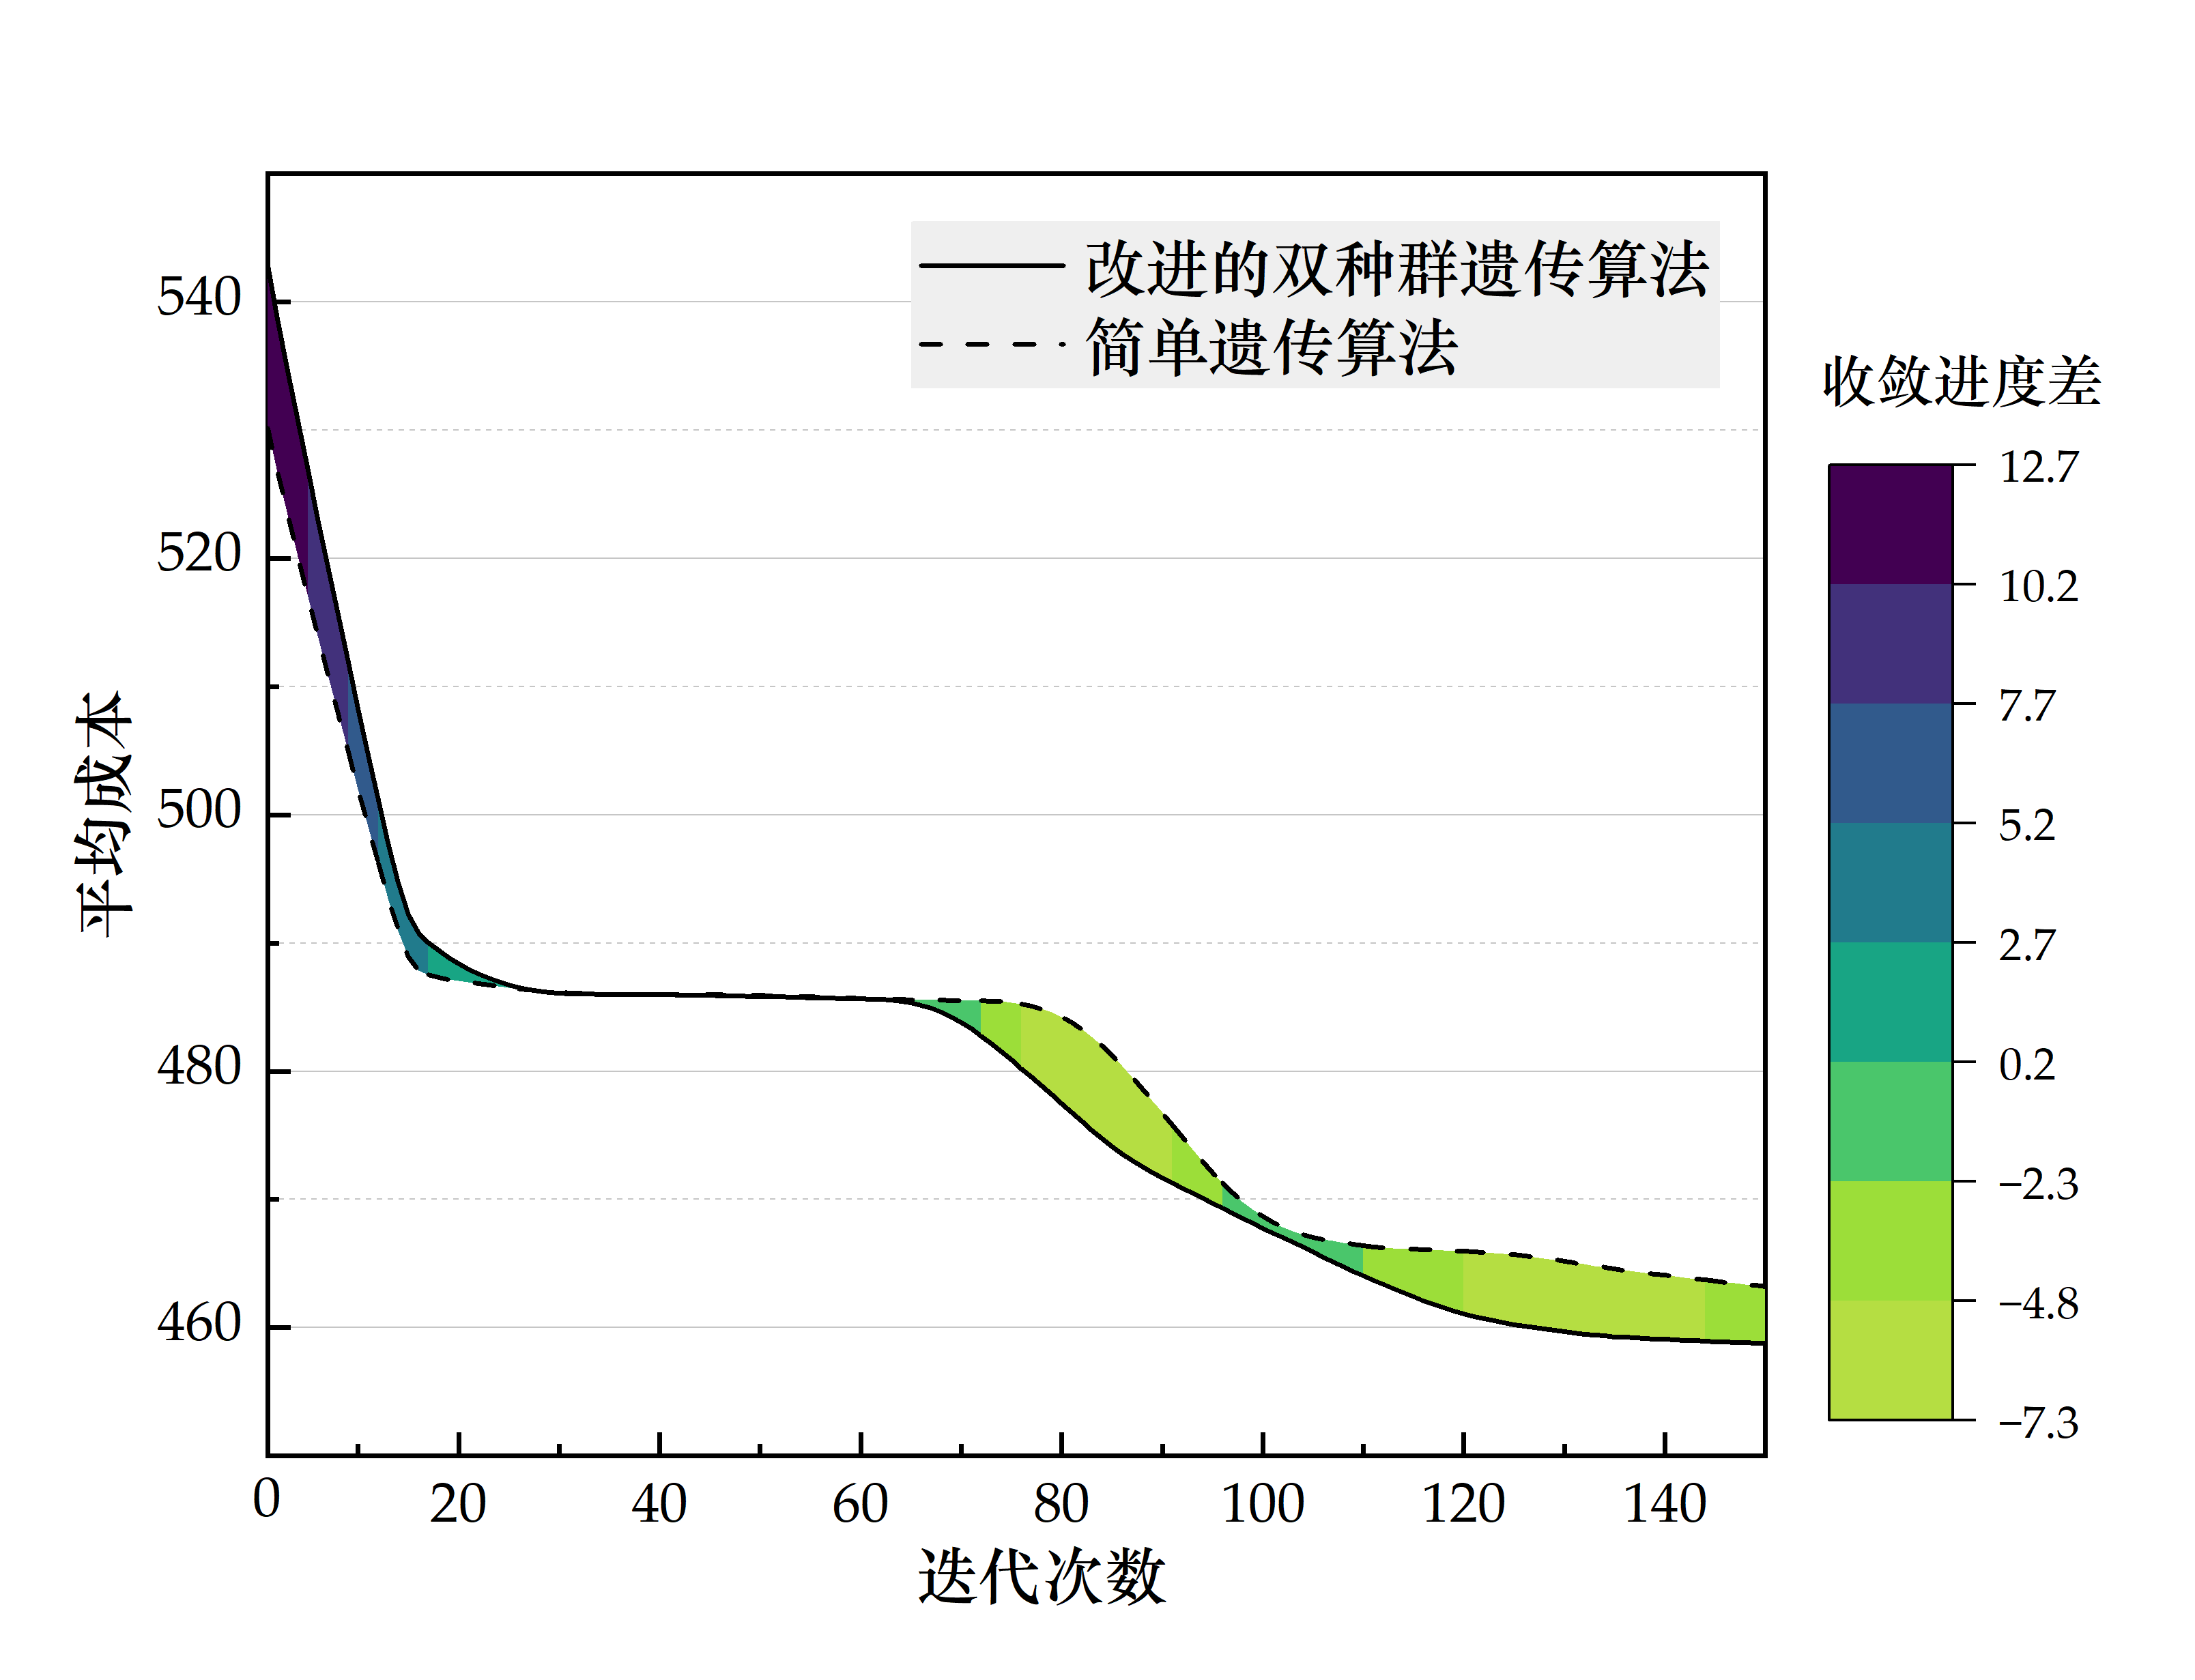
\includegraphics[width=1\linewidth]{CUMCMThesis-master//figures/算法比较.png}
            \caption{两种算法收敛效率和效果对比}
            \label{fig:algocmp}
        \end{minipage}
        \begin{minipage}[t]{0.49\linewidth}
            \centering
            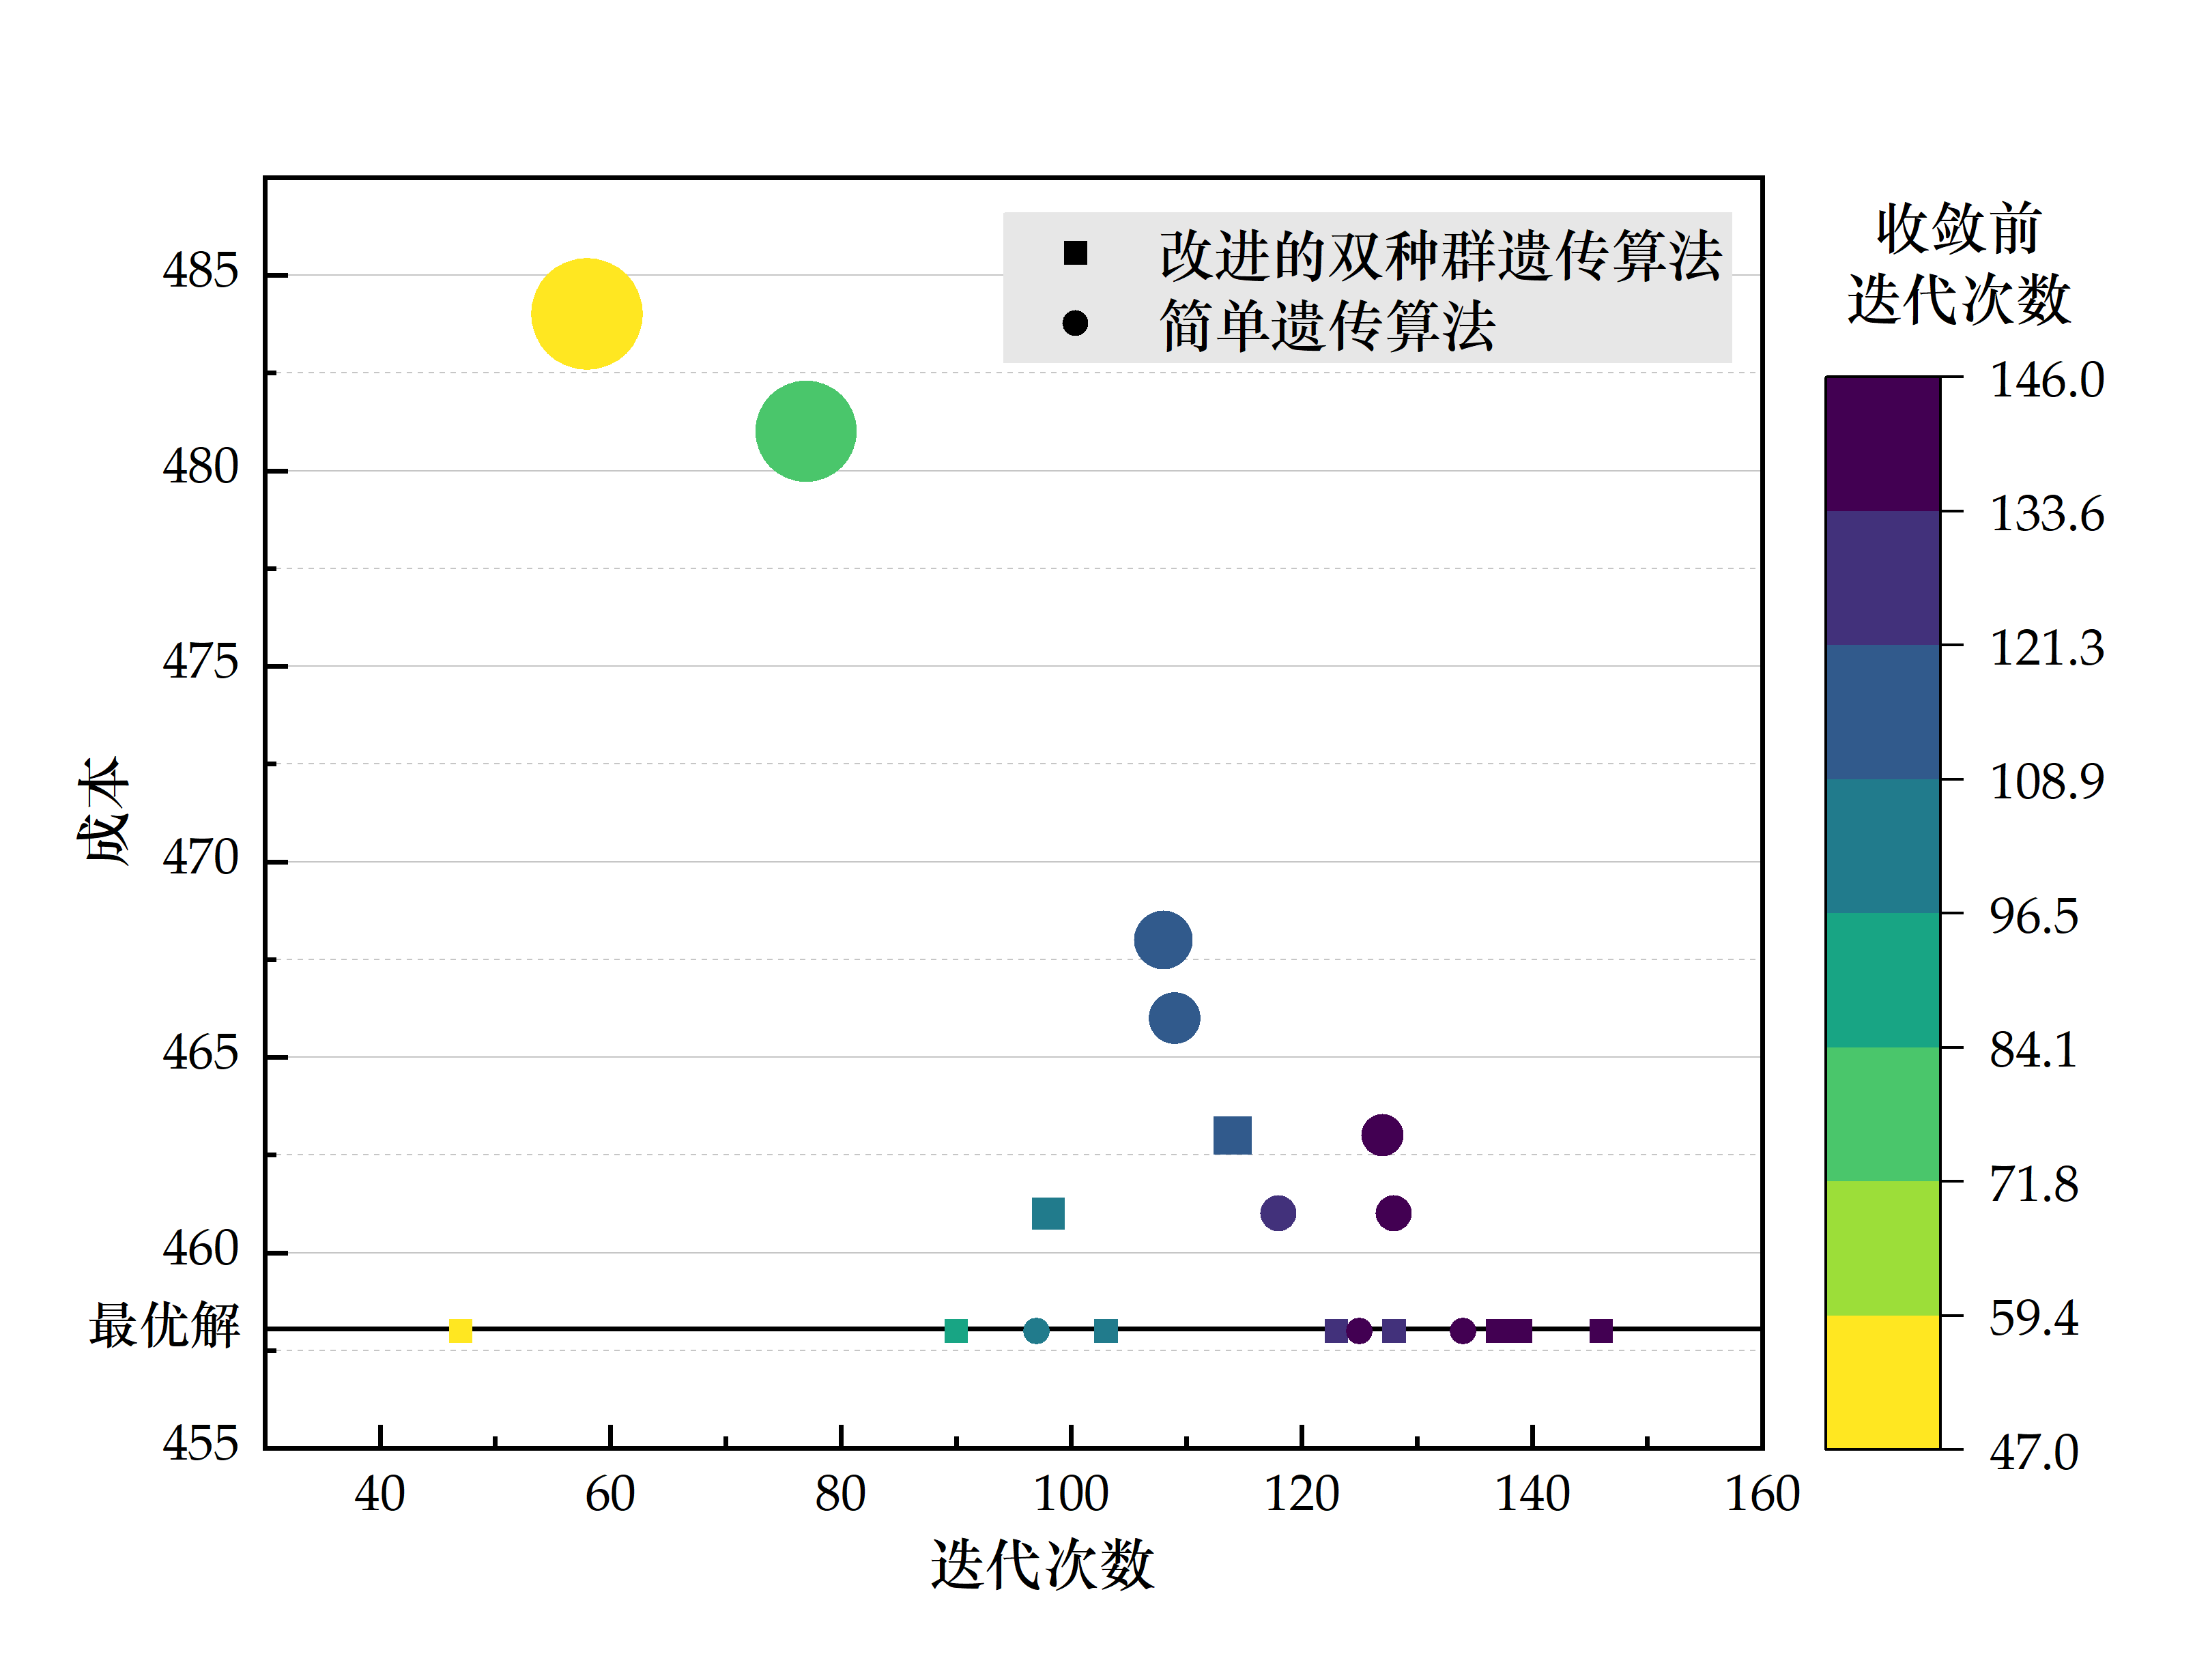
\includegraphics[width=1\linewidth]{CUMCMThesis-master//figures/稳定性.png}
            \caption{两种算法收敛结果稳定性对比}
            \label{fig:algocmp1}
        \end{minipage}
    \end{figure}
    \item \textbf{结果稳定性}。设置算法终止条件为连续80代不再出现更优解,分别进行10次实验,得到两种算法最终得到的成本和收敛起始点的散点图如图\ref{fig:algocmp1}。显然,改进后的双种群遗传算法具有更强的稳定性,早熟现象出现较少,收敛效率也略优于简单遗传算法。
\end{enumerate}

\subsection{模型评价与改进方向}

结合上述测试,总结模型的优势如下:
\begin{enumerate}
    \item 算法的收敛效率明显胜过简单遗传算法,且早熟情况明显减少,适合用于进行类似优化问题的训练;
    \item 提出了一种改进的双种群遗传算法,实现方式简单且效果尚佳;
    \item 运用自适应交叉率和变异率,且针对问题创新地给出了基于Bayes公式干预的变异概率控制。
\end{enumerate}

此外,该模型仍然存在一些有待改进之处,如纯粹的基于平均成本的单目标优化会导致所得答案普适性不高,对测试集效果远不及训练集,存在广义的“过拟合”情况;每次运算时仍有一定概率出现早熟的情况。对此,可以将问题转化为多目标优化问题,采用层次分析法,并设置动态权重以提高结果的普适性;可以考虑其他优化算法,如模拟退火算法、粒子群算法等,一定程度上避免早熟问题的出现。

\section{拓展研究:关于“选择”的算法优劣}
除了交叉、变异概率和种群规模等参数之外,选择算法的选取同样对整体算法有至关重要的影响。对当前优秀个体的过度选择容易陷入局部最优,而一味维持个体多样性则会拖慢收敛速度。为了解针对本问题的较优选择算法,进行以下研究。轮盘赌算法在前文中已经经过讨论,故在此不作介绍。

\subsection{待研究的选择算法}

\subsubsection{锦标赛选择(Tournament Selection)}

该算法进行若干次“锦标赛”(本题中次数即种群规模),每次有放回地从种群中随机取出k个个体,并将其中的最佳个体放入新种群。为了避免过高的重复度,往往设置较小的k(如2,3)。相对于以轮盘赌算法为代表的适应度值比例选择算法,锦标赛选择算法噪声较小,最优个体在其参与的所有竞赛中都会获胜,而最劣个体永远不会获胜。算法示意如图\ref{fig:tnmt}。

\begin{figure}[htbp]
    \centering
    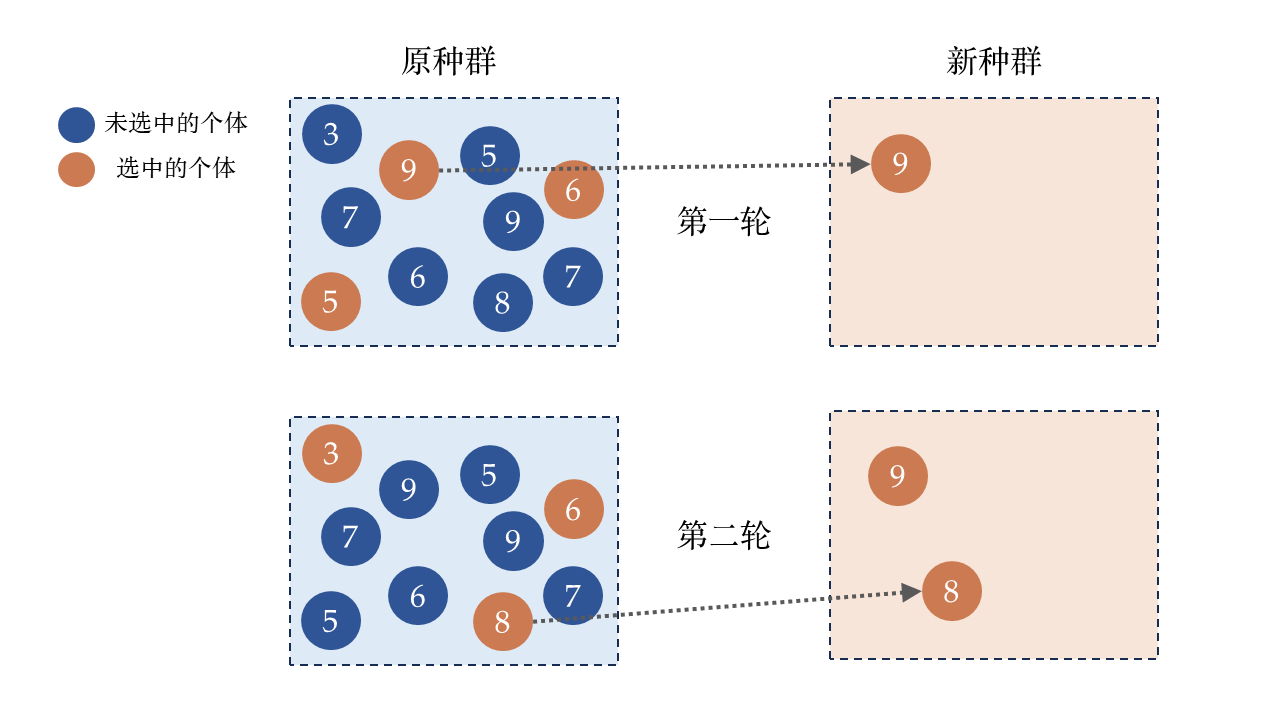
\includegraphics[width=0.75\linewidth]{CUMCMThesis-master//figures/锦标赛.png}
    \caption{k=3的锦标赛选择前两轮}
    \label{fig:tnmt}
\end{figure}

\subsubsection{截断选择(Truncation Selection)}

该算法较为朴素,直接在当前种群中重复选取适应度值为前k的个体,直至达到需要的新种群规模。该算法噪声为零,理论收敛速度最快,而对于较小的种群,容易导致多样性极小。但本题中,需要的种群规模较大(见\ref{sec:popsize}),故可以选取较多个体,实际操作中不一定显著弱于其他算法。

\subsubsection{随机遍历选择(Stochastic Universal Sampling, SUS)}

该算法是对轮盘赌算法的一个改变。为了丰富多样性,进一步提升不公平性以保留存在潜力的劣势个体,此算法在累计适应度值的基础上等间距取值。具体实现方法为:

\begin{enumerate}
    \item 计算取值间距$p=\sum^{N}_{i=1}f(x_i)/N$
    \item 在$[0,p)$范围内随机取值作为起始指针$p_0$
    \item 计算所有指针的位置,即$p_0,p_0+p,p_0+2p,\cdots ,p_0+(N-1)p$
    \item 根据指针位置在累计适应度中找到对应的个体,放入新种群
\end{enumerate}

这种算法相当于对多次随机过程进行了规范,理论上是对轮盘赌算法的一种优化。

\subsection{不同算法的比较实验}

虽然不同的算法在时间复杂度上有显著区别,但由于本问题的主要时间消耗在于三次样条插值而非遗传算法中的主干操作,故此处可以忽略。因此,仅针对本题,对上述算法的收敛效率、结果稳定性进行实验。

%【各个算法的收敛过程图(150代)】
为了更好地评价不同选择算法的收敛效率、结果稳定性,需要对两者进行规范化。收敛效率一般由达到某一成本值以下所需代数评判,而结果稳定性一般考虑收敛到最优解的频率。综合考虑之前的实验中得到的经验,定义收敛效率$\nu$和结果稳定性$\varsigma$如下:

\begin{itemize}
    \item 收敛效率$\nu$为10次实验的平均历史成本函数首次低于480所对应的迭代次数的倒数。
    \item 结果稳定性$\varsigma$为10次实验中收敛到458.9685次数占总实验次数的比例。
\end{itemize}

采用上述改进的双种群遗传算法,设置单个种群规模为200,代数为150,对四种算法分别进行10次测试。测试平台为Intel Core i7-12700H, Matlab R2023b和Intel Core i9-14900K, Matlab R2023b。测试结果如图\ref{fig:select},各算法的$\nu,\ \varsigma$值及其排名如表\ref{tab:select}。

\begin{figure}[htbp]
    \centering
    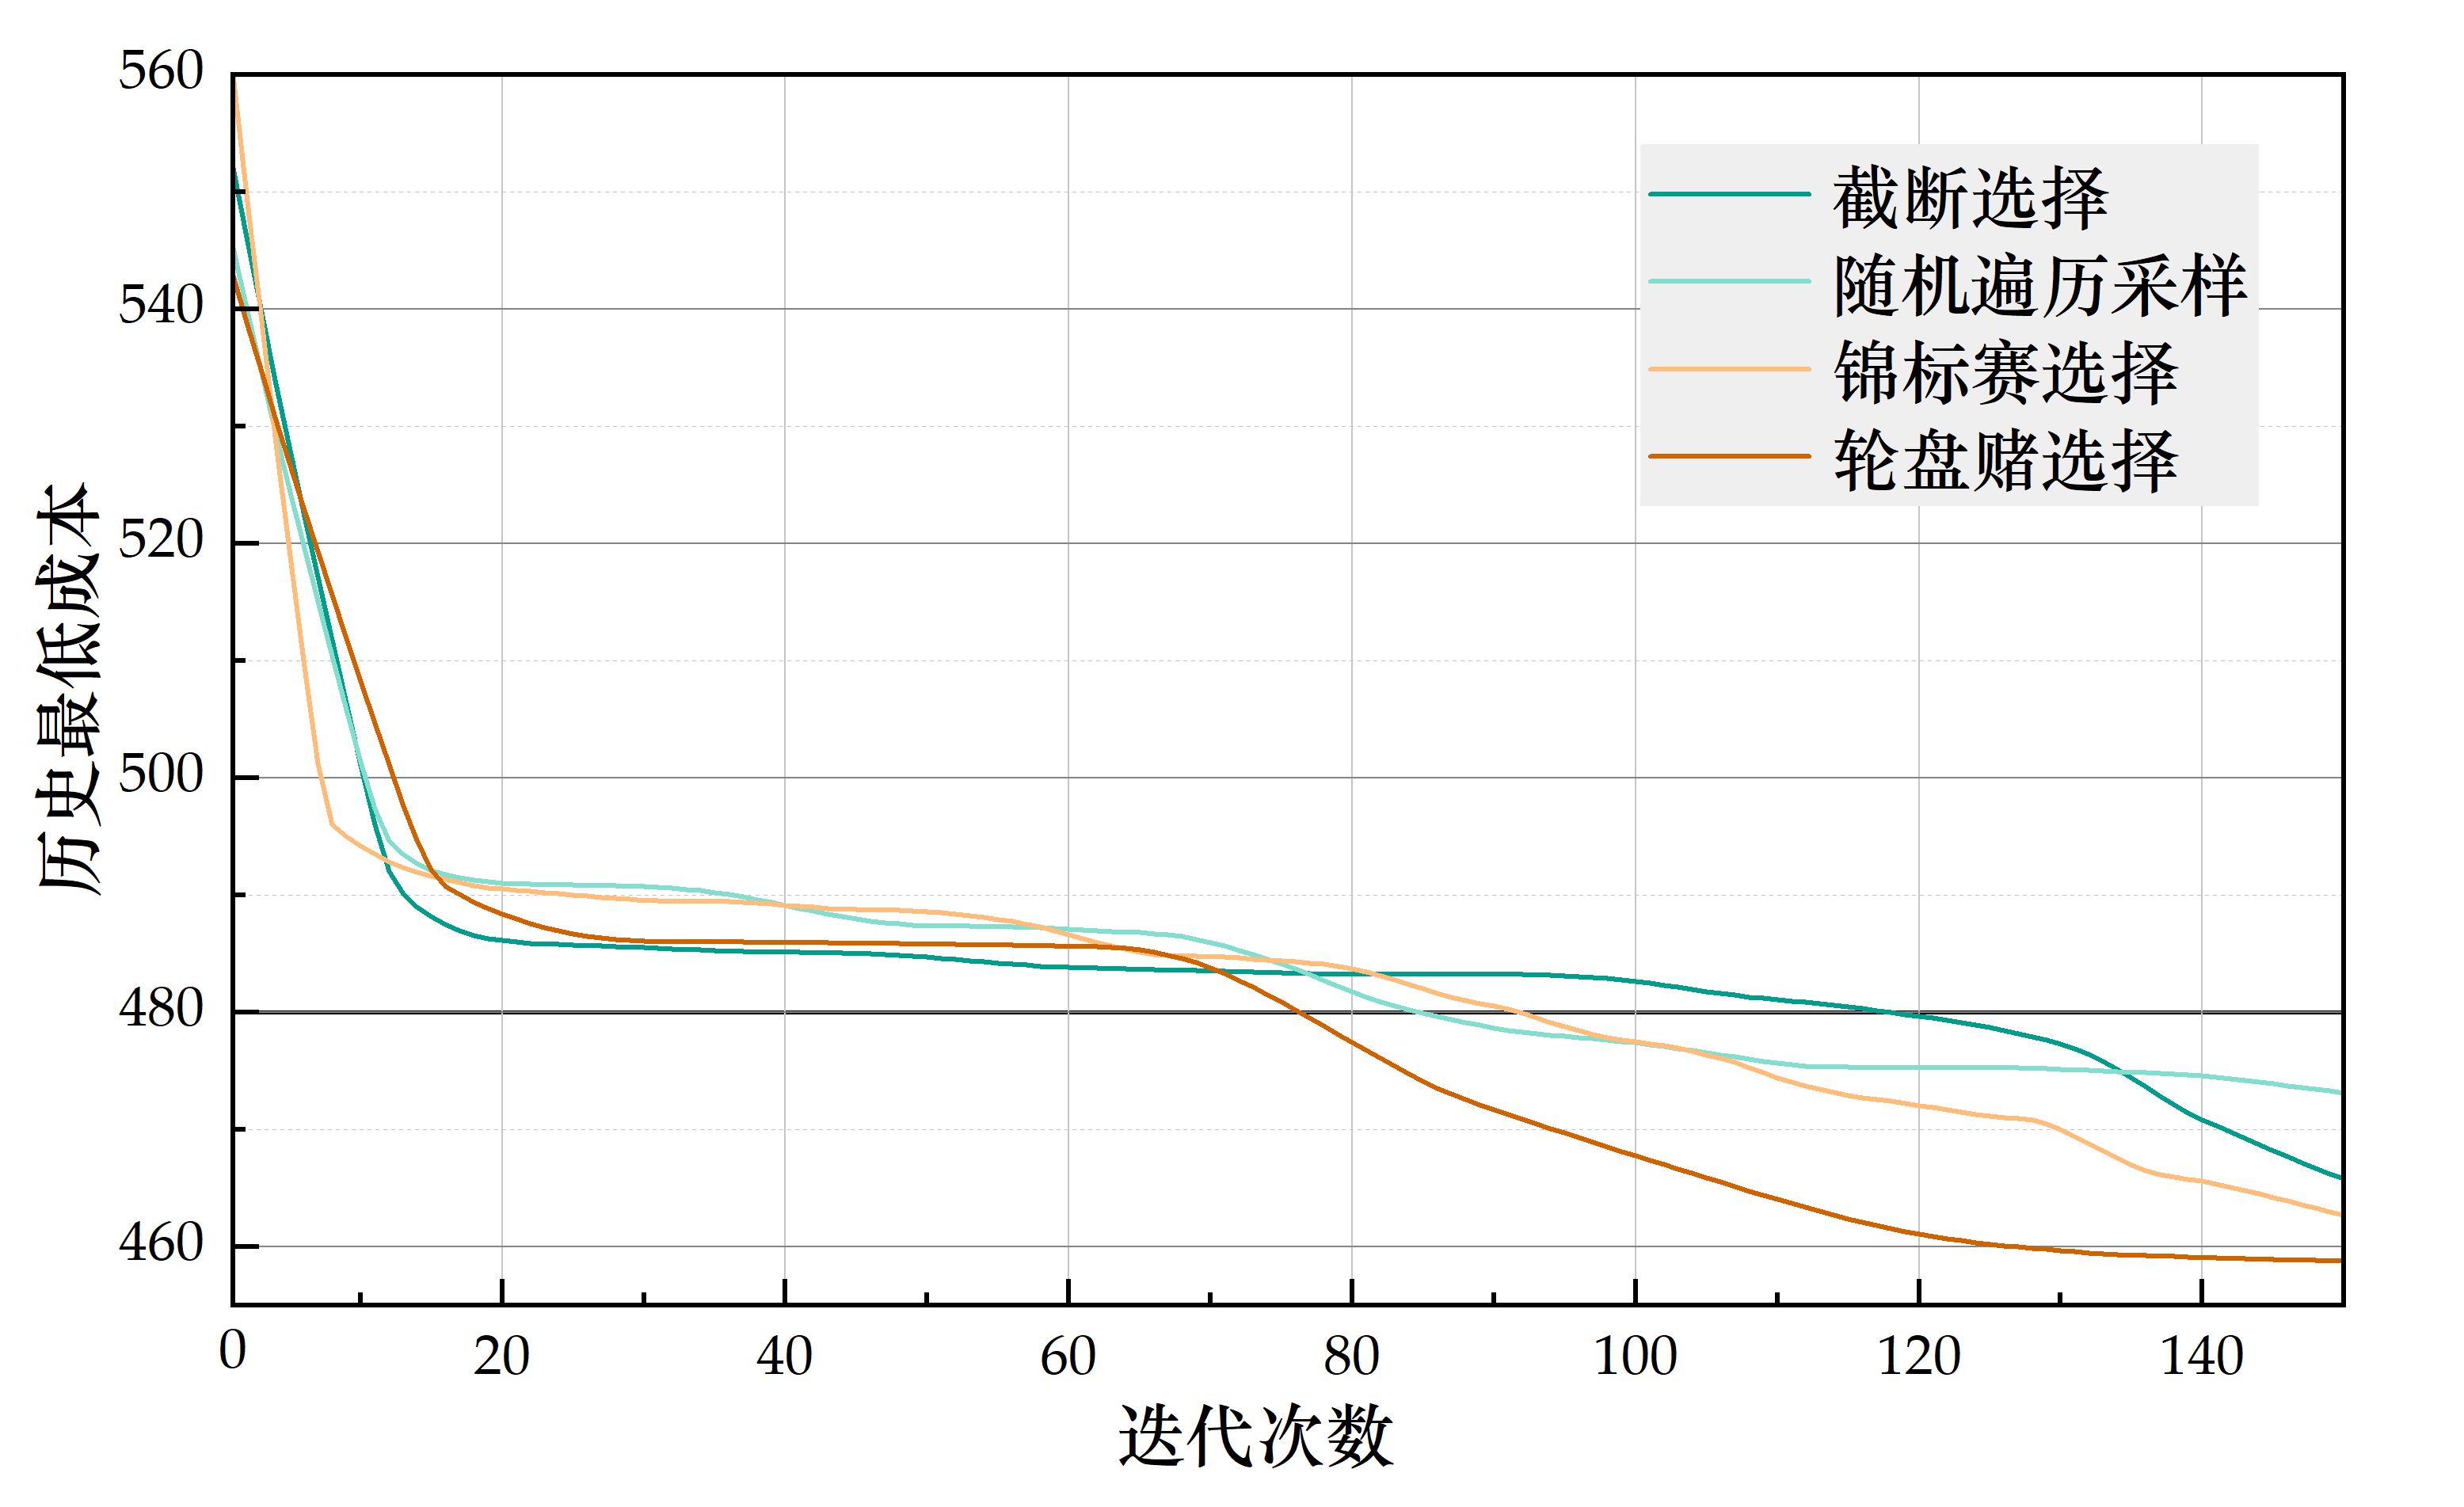
\includegraphics[width=0.62\linewidth]{CUMCMThesis-master//figures/选择算法效率.png}
    \caption{四种选择算法收敛情况对比}
    \label{fig:select}
\end{figure}

\begin{table}[htbp]
    \centering
    \caption{四种选择算法收敛效率及结果稳定性}
    \begin{tabular}{ccccc}
    \toprule
        选择算法 & 收敛效率$\nu$ & 结果稳定性$\varsigma$ & 收敛效率排名 & 结果稳定性排名 \\
    \midrule
        轮盘赌选择 & $13.0\times 10^{-3}$ & 0.7 & 1 & 1\\
        锦标赛选择 & $10.9\times 10^{-3}$ & 0.5 & 3 & 2\\
        截断选择 & $8.40\times 10^{-3}$ & 0.5 & 4 & 2\\
        随机遍历选择 & $11.8\times 10^{-3}$ & 0.3 & 2 & 4\\
    \bottomrule
    \end{tabular}
    \label{tab:select}
\end{table}

\subsection{实验结果分析}

本次实验与理论分析结果有所出入。轮盘赌选择在本题中仍然是四者中最优;随机遍历选择理论上优于轮盘赌算法,却在实际情况下结果稳定性较差;截断选择十分朴素,选择方法激进,却在收敛效率上表现不佳,反而在结果稳定性上表现尚可。这些情况的原因分析如下:

\begin{enumerate}
    \item 受限于算力和时间限制,未能进行足够次数的实验,结果仍然存在一定的偶然性;
    \item 遗传算法本身是一种以随机为根本的算法,每次实验之间都存在较大的数据差别,个别组的严重早熟状况会导致多组平均值的较大偏差,使得数据不能完全反映算法的表现;
    \item 每种算法本身没有绝对的优劣之分,在本题中表现的排名不能代表所有情况,使用改进的双种群遗传算法和使用简单遗传算法也可能得到不同的实验结果;
    \item 前述所有优化都是在轮盘赌选择算法的背景下进行的,如果更换选择算法,可能需要相应地更改其他参数。遗传算法的不同环节看似分立,实则环环相扣。
\end{enumerate}

依然可以确定的是,轮盘赌选择是针对解决本问题较好的一种选择算法;其他选择算法虽然表现不及轮盘赌算法,但同样可以通过重复试验得到相同的最优解。

%【对效率和稳定性进行量化,并进行可视化】
%【结合本题情况进行结果分析(为什么SUS不行,注意不要太确切因为你其实不知道为什么)】

\begin{thebibliography}{9}%宽度9
    \bibitem[1]{spline}
    许小勇,钟太勇.
    \newblock 三次样条插值函数的构造与Matlab实现\allowbreak[J].
    \newblock 兵工自动化,2006,(11):76-78.
    \bibitem[2]{dualpop}
    欧阳飞羽,王巍.
    \newblock 基于改进双种群遗传算法的装配线平衡优化研究\allowbreak[J].
    \newblock 中国新技术新产品,2023(23):118-121.
    \newblock DOI:10.13612/j.cnki.cntp.2023.23.030.
    \bibitem[3]{selfadapt}
    黄哲,颜廷旭.
    \newblock 基于自适应遗传算法的柔性机械手抑振轨迹优化\allowbreak[J].
    \newblock 工业控制计算机,2023,36(11):121-123.
    \bibitem[4]{canshu}
    熊邦书,黄武涛,李新民.
    \newblock 基于改进遗传算法的摄像机标定参数优化方法\allowbreak[J].
    \newblock 半导体光电,2016,37(01):110-114+118.
    \newblock DOI:10.16818/j.issn1001-5868.2016.01.024.
\end{thebibliography}

\newpage
%附录
\begin{appendices}

\section{核心代码片段}

\subsection{改进的双种群遗传算法主程序}
\begin{lstlisting}
clear;
n=90;
pop_size=200;
gens=150;

%初始化
pop1=round(rand(pop_size,n).^15);
pop2=round(rand(pop_size,n).^15);
pop1=logical(pop1);                   % logical减小内存占用,可能提升效率
pop2=logical(pop2);
%适应度记录
prev_best_fit=zeros(gens,1);
prev_avg_cost=zeros(gens,1);

for gen=1:gens
    disp(['正在进行第',num2str(gen),'次迭代']);
    %评估
    fit_val1=arrayfun(@(index) fitness(pop1(index,:)),1:pop_size)';
    [best_fit1,bestIdx1]=max(fit_val1);
    best_indiv1=pop1(bestIdx1,:);
    fit_val2=arrayfun(@(index) fitness(pop2(index,:)),1:pop_size)';
    [best_fit2,bestIdx2]=max(fit_val2);
    best_indiv2=pop2(bestIdx2,:);
    
    %记录历史
    prev_best_fit(gen)=max(best_fit1,best_fit2);
    disp([1/best_fit1+400,1/best_fit2+400]);


    newpop1=false(size(pop1));
    newpop2=false(size(pop2));
    %选择
    %轮盘赌
    cumul_fit=cumsum(fit_val1)/sum(fit_val1);
    for i=1:pop_size
        selected=rand();
        selected_index=find(cumul_fit>=selected,1);
        newpop1(i,:)=pop1(selected_index,:);
    end
    cumul_fit=cumsum(fit_val2)/sum(fit_val2);
    for i=1:pop_size
        selected=rand();
        selected_index=find(cumul_fit>=selected,1);
        newpop2(i,:)=pop2(selected_index,:);
    end
    %锦标赛
    % selected_index1=TournamentSelection(fit_val1,3,pop_size);
    % selected_index2=TournamentSelection(fit_val2,3,pop_size);
    %截断选择
    % selected_index1=TruncationSelection(fit_val1,15,pop_size);
    % selected_index2=TruncationSelection(fit_val2,15,pop_size);
    %随机遍历选择
    % selected_index1=StochasticUniversalSampling(fit_val1,pop_size);
    % selected_index2=StochasticUniversalSampling(fit_val2,pop_size);
    % for i=1:pop_size
    %     newpop1(i,:)=pop1(selected_index1(i),:);
    % end
    % for i=1:pop_size
    %     newpop2(i,:)=pop2(selected_index2(i),:);
    % end
    
    %交叉
    f_avg1=mean(fit_val1);
    f_avg2=mean(fit_val2);
    prev_avg_cost(gen)=2/(f_avg2+f_avg1)+400;
    disp(prev_avg_cost(gen));
    for i=1:2:pop_size
        if min(fit_val1(i),fit_val1(i+1))<f_avg1
            cross_rate=1;
        else
            cross_rate=1-0.2*(fit_val1(i)-f_avg1)/(best_fit1-f_avg1);
        end
        if rand()<cross_rate
            t1=randi(n);t2=randi(n);
            cross_pnt_left=min(t1,t2);
            cross_pnt_right=max(t1,t2);
            newpop1(i,cross_pnt_left:cross_pnt_right)=newpop1(i+1,cross_pnt_left:cross_pnt_right);
            newpop1(i+1,cross_pnt_left:cross_pnt_right)=newpop1(i,cross_pnt_left:cross_pnt_right);
        end
        if min(fit_val2(i),fit_val2(i+1))<f_avg2
            cross_rate=1;
        else
            cross_rate=1-0.2*(fit_val2(i)-f_avg2)/(best_fit2-f_avg2);
        end
        if rand()<cross_rate
            t1=randi(n);t2=randi(n);
            cross_pnt_left=min(t1,t2);
            cross_pnt_right=max(t1,t2);
            newpop2(i,cross_pnt_left:cross_pnt_right)=newpop2(i+1,cross_pnt_left:cross_pnt_right);
            newpop2(i+1,cross_pnt_left:cross_pnt_right)=newpop2(i,cross_pnt_left:cross_pnt_right);
        end
    end
    
    %变异
    if gen==1
        mut_rate_ones=0.92;
        mut_rate_zeros=0.08;
    else
        mut_rate_zeros=sum(best_indiv1)/n;
        mut_rate_ones=1-mut_rate_zeros;
    end
    for i=1:pop_size
        if fit_val1(i)<f_avg1
            mut_rate=0.05*n/2/sum(best_indiv1);
        else
            mut_rate=(0.05-0.03*(fit_val1(i)-f_avg1)/(best_fit1-f_avg1))*n/2/sum(best_indiv1);
        end
        for j=1:n
            if newpop1(i,j)==true && rand()<mut_rate*mut_rate_ones || newpop1(i,j)==false && rand()<mut_rate*mut_rate_zeros
                newpop1(i,j)=~newpop1(i,j);
            end
        end
    end
    newpop1(1,:)=best_indiv1;

    if gen==1
        mut_rate_ones=0.92;
        mut_rate_zeros=0.08;
    else
        mut_rate_zeros=sum(best_indiv2)/n;
        mut_rate_ones=1-mut_rate_zeros;
    end
    for i=1:pop_size
        if fit_val2(i)<f_avg2
            mut_rate=0.05*n/2/sum(best_indiv2);
        else
            mut_rate=(0.05-0.03*(fit_val2(i)-f_avg2)/(best_fit2-f_avg2))*n/2/sum(best_indiv2);
        end
        for j=1:n
            if newpop2(i,j)==true && rand()<mut_rate*mut_rate_ones || newpop2(i,j)==false && rand()<mut_rate*mut_rate_zeros
                newpop2(i,j)=~newpop2(i,j);
            end
        end
    end
    newpop2(1,:)=best_indiv2;
    
    %移民
    if rem(gen,5)==0
        newpop2(find(fit_val2==min(fit_val2),1),:)=best_indiv1;
        newpop1(find(fit_val1==min(fit_val1),1),:)=best_indiv2;
    end

    %table=array2table(newpop);
    %writetable(table,'newpop.xlsx');
    %table=array2table(pop);
    %writematrix(pop,'pop.xlsx');
    %更新种群
    pop1=newpop1;
    pop2=newpop2;
end

disp('最优选择:');
if best_fit1>best_fit2
    best_indiv=best_indiv1;
    cost=1/best_fit1+400;
else
    best_indiv=best_indiv2;
    cost=1/best_fit2+400;
end
disp(find(best_indiv));
disp(['最低成本:' num2str(cost)]);
prev_low_cost=1./prev_best_fit+400;
%table=array2table(prev_low_cost);
%writetable(table,'选择-SUS.xlsx');
x=1:gens;
plot(x,prev_low_cost,'-*b',x,prev_avg_cost,'-or');
axis([0,160,400,2400])
set(gca,'XTick',0:20:160)
set(gca,'YTick',400:400:2400)
legend('最低成本','平均成本');
xlabel('x')
ylabel('y')
\end{lstlisting}

\subsection{适应度计算函数}

\begin{lstlisting}
function fitness=fitness(individual)
    % 只读取一次数据提高效率
    persistent data;
    if isempty(data)
        table=readtable("dataform_train2024.csv");
        data=table2array(table);
    end
    
    % 三次样条插值、多项式拟合
    datanum=2000;
    X=find(individual);
    len=length(X);
    if len<2
        fitness=0;
        return;
    end
    yi=data(2:2:2*datanum,1:90);
    y=data(2:2:2*datanum,X);
    V=zeros(datanum,90);
    for i=1:datanum
        V(i,:)=interp1(y(i,:),X,yi(i,:),'spline');
    end
    %table=array2table(Y);
    %writetable(table,"Y.csv");

    % 成本计算
    fitness=80*length(X);
    delta=abs(V-(1:90));
    %disp(delta);
    s1=sum(sum(delta>0.5));
    s2=sum(sum(delta>1))*9;
    s3=sum(sum(delta>1.5))*20;
    s4=sum(sum(delta>2))*79970;
    fitness=fitness+(s1+s2+s3+s4)/datanum;
    fitness=1/(fitness-400);    % -400,突出优质个体的适应度优势,提高收敛速度

end
\end{lstlisting}

\subsection{锦标赛选择、截断选择、随机遍历选择算子}

\begin{lstlisting}
% 锦标赛选择
function [selected_indices] = TournamentSelection(fitness, tournamentSize, numSelected)
    populationSize = length(fitness);
    selected_indices = zeros(1, numSelected);
    
    for i = 1:numSelected
        tournamentContestants = randperm(populationSize, tournamentSize);
        [~, bestIndex] = max(fitness(tournamentContestants));
        winner = tournamentContestants(bestIndex);
        selected_indices(i) = winner;
    end
end
%截断选择
function [selected_indices] = TruncationSelection(fitness, selection, pop_size)
    sorted=sort(fitness);
    selected_indices=zeros(1,pop_size);
    for i=1:pop_size
        selected_indices(i)=find(fitness==sorted(pop_size-rem(i-1,selection)),1);
    end
end
%随机遍历选择
function selected = StochasticUniversalSampling(fitness,pop_size)
    [ind,~] = size(fitness);
    cumfit = cumsum(fitness);
    trials = cumfit(ind) / pop_size * (rand + (0:pop_size-1)');
    f = cumfit(:, ones(1, pop_size));
    t = trials(:, ones(1, ind))';
    [selected, ~] = find(t < f & [ zeros(1, pop_size); f(1:ind-1, :) ] <= t);
    [~, shuf] = sort(rand(pop_size, 1));
    selected = selected(shuf);
end
\end{lstlisting}

\end{appendices}

\end{document} 